\chapter{Sensors for Attitude Determination}

The attitude of the satellite is measured and estimated in order to control it and a sufficient amount of sensors has to be implemented to get the necessary accuracy on the estimated attitude. The main sensors used for attitude determination are star trackers, horizon sensors, sun sensors, GPS antenna arrays, magnetometers and angular rate gyroscopes.We use Magnetometer, Sun sensors and Gyroscopes for attitude determination. 


\section{Magnetometer}

A magnetometer is a scientific instrument used to measure the strength and direction of the magnetic field in the vicinity of the instrument. The magnetometer, also known as a magnetic sensor, is an important sensor component in all types of aircraft and spacecraft. In the field of aeronautics, the magnetometer can be used to measure the geomagnetic field vector information of the position of the aircraft body, such as airplanes and satellites. And, according to the reference model for the Earth’s magnetic field and local magnetic field, the angle information of a certain precision can be obtained through an algorithm, therefore, the magnetometer is widely used in aircraft attitude determination systems, especially in microsatellites, such as nanosatellites and picosatellites, etc.


\begin{figure}[h!]
	\centering
	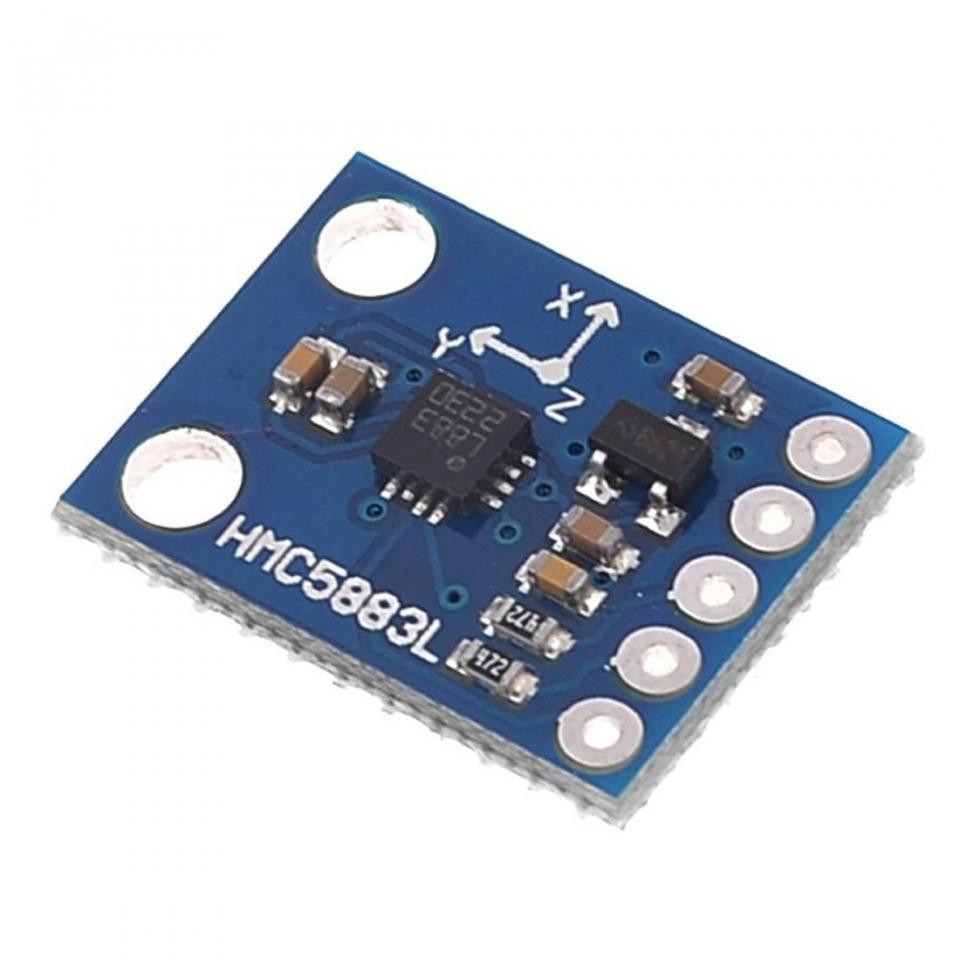
\includegraphics[width=3in,height=2.5in]{./images/magnetometer.jpg}
	\caption{Magnetometer}
	\label{magnetometerimg}
\end{figure}


\subsection{Working Principle}

Earth’s magnetic field is present in space which points towards the magnetic north as shown in below image. Current carrying conductor also generates a magnetic field around itself. Hence, whenever a current carrying conductor is placed in space, it experiences the effect of the earth’s magnetic field affecting the flow of the electrons through that conductor. These changes in the flow of the electrons are used for identifying the heading or direction of the magnetic field. This is the basic working principle of the magnetometer.

\begin{figure}[h!]
	\centering
	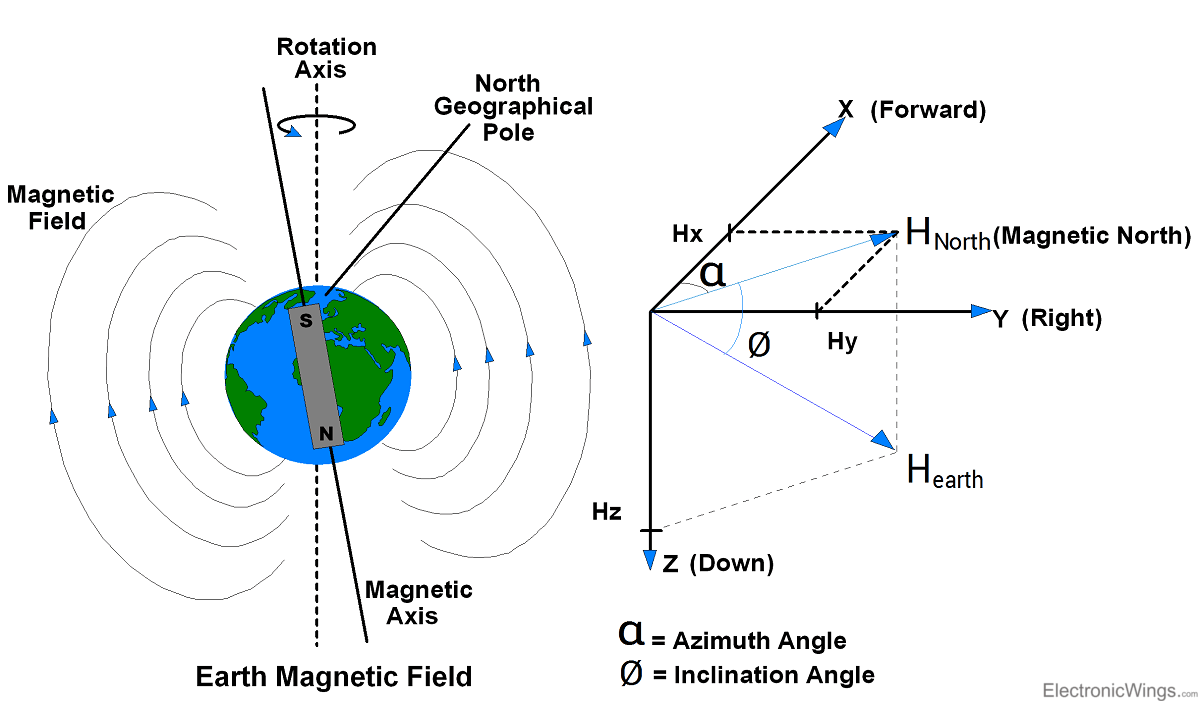
\includegraphics[width=5.5in,height=3.22in]{./images/earthmf.png}
	\caption{Earth's Magnetic field}
	\label{earthmfimg}
\end{figure}

\section{Sun sensor}

A sun sensor is a navigational instrument used by spacecraft to detect the position of the sun. Sun sensors are used for attitude control, solar array pointing, gyro updating, and fail-safe recovery. Sun sensors are widely used in spacecraft attitude determination systems for measuring the sun vector in spacecraft coordinates. Sun sensor determines a spacecraft’s orientation with respect to the sun.

\begin{figure}[!h]
	\centering
	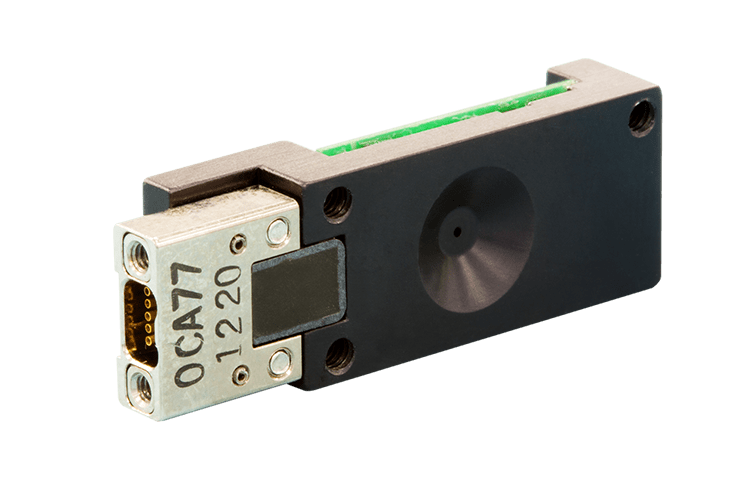
\includegraphics[width=3.5in,height=2.5in]{./images/sunsensor.png}
	\caption{Sun sensor}
	\label{sunsensorimg}
\end{figure}


\subsection{Working Principle}

The sun sensor is operated based on the entry of light into a thin slit on top of a rectangular chamber whose bottom part is lined with a group of light-sensitive cells. The chamber casts an image of a thin line on the chamber bottom. The cells at the bottom measure the distance of the image from a centerline and determine the refraction angle by using the chamber height.
The cells are operated based on the photoelectric effect. They convert the incoming photons into electrons and hence voltages which are in turn converted into a digital signal. When two sensors are placed perpendicular to each other, the direction of the sun with reference to the sensor axes can be calculated.

\vspace{15pt}

The solar cells provide a current output depending on the angle made by the sensor normal with the sun vector based on cosine law,

$$I = I_0 cos(\theta)$$
where $I_0$ is the intensity at zero angle.

\begin{figure}[!h]
	\centering
	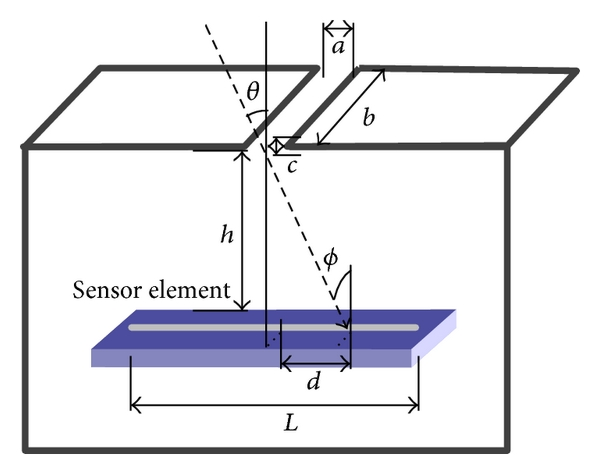
\includegraphics[width=2.5in,height=2in]{./images/sun sensor_w.jpg}
	\caption{Sun sensor working principle}
	\label{sunsensorw}
\end{figure}


\section{Gyroscope}

A gyroscope is a device used for measuring or maintaining orientation and angular velocity. It is a spinning wheel or disc in which the axis of rotation (spin axis) is free to assume any orientation by itself. When rotating, the orientation of this axis is unaffected by tilting or rotation of the mounting, according to the conservation of angular momentum.

\begin{figure}[h!]
	\centering
	\begin{subfigure}[b]{0.45\textwidth}
		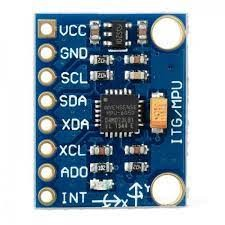
\includegraphics[width=\textwidth,height=2in]{./images/Gyro.jpeg}
		\caption{Gyroscope}
		\label{gyro-1}
	\end{subfigure}
	\begin{subfigure}[b]{0.45\textwidth}
		\centering
		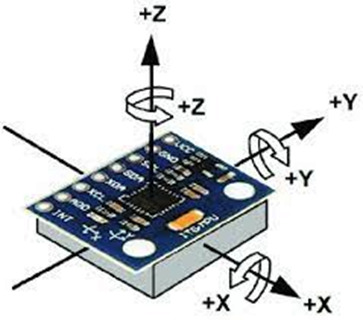
\includegraphics[width=\textwidth,height=2in]{./images/Gyro2.jpeg}
		\caption{MPU 6050}
		\label{gyro-2}
	\end{subfigure}
\end{figure}

\subsection{Working Principle}

Depending on the direction there are three types of angular rate measurements. Yaw- the horizontal rotation on a flat surface when seen the object from above, Pitch- Vertical rotation as seen the object from front, Roll- the horizontal rotation when seen the object from front.
The concept of Coriolis force is used in Gyroscope sensors. In this sensor to measure the angular rate, the rotation rate of the sensor is converted into an electrical signal. 
This sensor consists of an internal vibrating element made up of crystal material in the shape of a double – T- structure. This structure comprises a stationary part in the centre with ‘Sensing Arm’ attached to it and ‘Drive Arm’ on both sides.
This double-T-structure is symmetrical. When an alternating vibration electrical field is applied to the drive arms, continuous lateral vibrations are produced. As Drive arms are symmetrical, when one arm moves to left the other moves to the right, thus cancelling out the leaking vibrations. This keeps the stationary part at the centre and sensing arm remains static.
When the external rotational force is applied to the sensor vertical vibrations are caused on Drive arms. This leads to the vibration of the Drive arms in the upward and downward directions due to which a rotational force acts on the stationary part in the centre.
Rotation of the stationary part leads to the vertical vibrations in sensing arms. These vibrations caused in the sensing arm are measured as a change in electrical charge. This change is used to measure the external rotational force applied to the sensor as Angular rotation. Besides sensing the angular velocity, Gyroscope sensors can also measure the motion of the object. 




